\chapter{绪论}
\vspace{7pt}

本章作为全文的开篇，首先阐述自动化用例建模研究的背景与意义，分析传统手工建模方式的局限性以及大语言模型带来的技术机遇；随后梳理国内外在基于自然语言处理的建模技术、大语言模型驱动的建模方法以及多智能体系统应用等方面的研究现状；在此基础上，提出本文的研究内容与主要创新点；最后说明论文的整体组织结构。

\section{研究背景与意义}

\subsection{软件开发全生命周期中需求分析的重要性}

需求分析是软件开发生命周期中最为关键的起始阶段。在当今大规模复杂软件系统的开发实践中，需求文档的篇幅常常达到数百页，一份完整的需求规格说明书可能涵盖数十个功能模块和上百个业务场景。手工阅读和分析的方式不仅耗时巨大，还容易因分析师的认知负荷与经验差异导致关键信息的遗漏。传统手工分析模式已难以适应现代软件工程的规模和复杂度要求。因此，探索智能化、自动化的用例建模方法对于提升软件工程实践效率具有重要的现实意义。

\subsection{传统手动UML建模的低效性与语义偏差问题}

传统的UML建模工作高度依赖人工操作。系统分析师需要逐段阅读需求文档，手工识别出系统参与者、用例以及它们之间的各类关系，随后在建模工具中逐一绘制图形元素。这一过程存在若干固有缺陷。

首先，手工建模效率低下。当需求文档篇幅较长时，分析师需要反复翻阅文本以确保不遗漏关键信息，阅读与绘图之间的频繁切换进一步降低了工作效率。对于需要迭代修改的需求版本，重新调整模型图的工作量几乎等同于从零开始。

其次，不同分析师的认知差异会引入语义偏差。Cámara等人\cite{camara2023assessment}通过八组独立的UML建模实验证实，即便是人类专家之间，对于同一需求描述的建模结果也存在显著差异，这反映了手工建模固有的主观性问题。例如，某业务流程的某些环节可能被一位分析师识别为独立用例，而另一位分析师则将其归入主流程的扩展路径，这种不一致性直接影响了后续设计开发活动对需求理解的准确传递。

\subsection{大语言模型在代码生成与语义理解中的突破}

以Transformer架构为核心的大语言模型通过在海量文本语料上的预训练，获得了强大的语义理解与文本生成能力\cite{vaswani2017attention}。模型不仅能够理解自然语言中的显式信息，还能在一定程度上推理文本中隐含的逻辑关系。

在代码生成领域，基于大语言模型的工具已展现出从自然语言描述直接生成可执行代码的能力。然而，UML模型作为一种图形化的语义表达形式，其生成任务对模型的结构化输出能力提出了更高要求。Ferrari等人\cite{ferrari2024model}在从结构化需求生成UML时序图的研究中发现，大语言模型生成的模型虽然在语法层面基本符合UML标准，但在完整性和正确性方面仍存在明显不足，尤其当需求描述包含歧义时表现更不稳定。戴莉萍和王文乐在UML建模实验研究中也探讨了文本驱动建模方式在可维护性方面的优势\cite{dailiping2021}。

将大语言模型引入用例建模流程，有望从根本上改变传统的手工建模模式。模型可以快速处理长篇幅的需求文档，自动抽取关键实体并分析其间的语义关联，从而大幅提升建模效率。同时，基于统一模型参数的分析过程可以消除不同人员之间的认知偏差。国内已有相关实践通过构建“需求感知-语义建模-动态验证”的全链路可视化流程，证明了将大语言模型的强大语义解析能力与 UML 可视化建模优势相结合，能够有效实现需求分析的智能化，并大幅提升软件需求规格说明书的编写质量\cite{yang2025software}。然而，单次大模型调用在处理复杂长文档时容易出现上下文窗口溢出和信息遗忘问题，如何在自动化建模中保证提取结果的完整性与准确性，仍是需要进一步研究的关键课题\cite{giannouris2025nomad}。

\section{国内外研究现状}

\subsection{基于自然语言处理规则的传统建模技术}

在深度学习技术大规模应用之前，研究者已开始探索利用自然语言处理技术从需求文本中自动生成UML模型。王飞等人\cite{wangfei2018}探索了将结构化自然语言需求转换为形式化模型的方法，但该方法高度依赖预定义的模板结构，对自由文本的适应能力有限。More和Phalnikar\cite{more2012generating}提出了基于词性标注和句法分析识别UML类名和关系的方法，受限于手工规则的覆盖范围和语言的固有歧义，在跨领域场景下泛化能力较弱。

基于规则和模板的方法虽然在特定受限场景下具有一定效果，但其通常高度依赖手工预设特征、领域词典或简单的关键词匹配，在处理同义词、跨段落逻辑以及复杂的隐含语义时存在显著的局限性\cite{meng2024automated, abdelnabi2020generating, zhaohuipan2021}。即便近期有研究尝试引入深度自然语言处理技术来提取需求文本的深层语义与时序特征，这类方法在底层的图元素抽取阶段依然未能完全摆脱对词性标注和句法依存等启发式人工规则的依赖\cite{yuan2026automatedadgc}。这种对规则的固有依赖，不仅极大限制了系统在跨领域场景下的泛化能力，也导致其难以胜任复杂业务逻辑下多类型UML图表的协同生成任务。

\subsection{基于Transformer架构的大语言模型建模研究现状}

随着预训练语言模型的兴起，基于大语言模型的自动化建模研究进入新阶段。在UML类图生成方面，Wang等人\cite{wang2024llms}调查了大语言模型辅助下本科生进行UML建模的效果，发现模型在类定义方面的准确率较高。De Bari等人\cite{debari2024evaluating}系统比较了不同大语言模型和提示策略在UML类图建模练习中的表现，初步验证了大语言模型在建模任务上的可行性。Fill等人\cite{fill2023conceptual}通过首次实验探索了ChatGPT在概念建模方面的表现，发现尽管语法正确性较高，但语义准确性仍需人工审查。

然而，现有研究也暴露出若干不足。Cámara等人\cite{camara2023assessment}在评估ChatGPT建模性能时发现，模型在生成十至十二个类以上的大型模型时会出现严重的语义错误，且输出在不同会话中存在高度不一致性。Chen等人\cite{chen2023automated}在2023年MODELS会议上评估了GPT系列模型在十个领域示例上的自动建模效果，尽管模型展示出令人满意的领域理解能力，但距离完全实现建模自动化仍有较大差距。此外，大多数研究仅聚焦于单一图表类型的生成，缺乏对多类型UML图表进行协同生成的系统级方案\cite{giannouris2025nomad,nguyen2026class}。

\subsection{多智能体在复杂逻辑推理中的应用}

多智能体系统通过多个专业化智能体的协作完成复杂任务，在逻辑推理、规划与问题求解领域展现出显著优势。任务分解、角色分工和通信协作是多智能体系统的三大核心机制。Li等人\cite{li2023camel}提出的CAMEL框架与Wu等人\cite{wu2023autogen}提出的AutoGen框架分别从不同角度探索了大规模语言模型在多智能体对话协作中的应用潜力。

在软件工程领域，Qian等人\cite{qian2023chatdev}提出的ChatDev框架将多智能体架构系统性地引入软件开发完整流程，通过定义产品经理、架构师、程序员等角色实现了分工协作，为该领域提供了开创性的研究范式。

在用例建模场景中，Giannouris与Ananiadou\cite{giannouris2025nomad}提出的NOMAD框架是目前最为系统的多智能体UML生成方案，其核心设计理念——将建模任务分解为概念提取、关系理解、模型集成和代码生成四个专业化子任务——为本文的工作提供了直接的方法论基础。该研究的实验结果还表明，多智能体架构天然支持在关键节点插入人工审核的中断机制，为人机协同提供了灵活的工程框架。

\section{主要研究内容与创新点}

\subsection{构建基于LangGraph的多角色协同Agent建模管道}

本研究的第一个核心工作是设计并实现基于LangGraph的多智能体协作建模工作流。Giannouris与Ananiadou\cite{giannouris2025nomad}在NOMAD框架中提出了将UML类图生成任务分解为多个专业化子任务的认知启发式架构，验证了概念提取、关系理解、模型集成和代码生成四阶段流水线的有效性。本文借鉴了这一任务分解思想，并将其从类图扩展到用例图和时序图的生成场景中，将UML图的生成过程分解为多个子任务，分别由独立的Agent节点承担。

在工作流的断点设计上，系统在关系分析节点执行之前设置中断点，允许用户在确认实体提取结果后再启动关系推理。ChatDev框架\cite{qian2023chatdev}同样验证了在关键决策点引入人工审查对保障输出质量的积极作用，本系统将这一机制应用于UML建模场景，既保留了自动化处理的效率，又赋予用户对关键中间结果的控制权。

\subsection{引入RAG技术解决长文档场景下的信息丢失与幻觉}

针对大语言模型在处理长文档时存在上下文窗口限制和信息遗忘的问题，本研究引入检索增强生成技术以提升提取质量。Nguyen等人\cite{nguyen2026novel}在自动化UML图生成统一框架中同样引入了RAG模块，验证了上下文增强在UML合成中的有效性。

本文采用ChromaDB作为向量数据库，利用Sentence-Transformers模型将需求文档的文本块转化为语义向量。当执行特定模块的用例提取任务时，系统首先通过语义检索从向量库中获取与该模块最相关的上下文段落，再将检索结果注入提示词中，使大语言模型获得聚焦的信息输入。RAG技术的应用有效缓解了两个关键问题。其一，通过检索机制突破了大模型上下文窗口对文本长度的限制，即使需求文档篇幅超出模型的最大输入长度，相关的核心信息依然能够通过检索被引入生成过程。其二，上下文增强的提示词使模型更倾向于基于原文信息进行推理，显著降低了幻觉现象发生的概率，提升了生成结果的忠实度。实验验证表明，RAG增强在跨模块实体一致性和跨模块关系完整性两个维度上均产生了一定的正向效果，但改善幅度有限，在检索质量控制和上下文筛选方面仍有优化空间。

\subsection{PlantUML渲染稳定性的模板清洗与逻辑约束算法}

大语言模型生成的PlantUML代码并非总是语法合法。Cámara等人\cite{camara2023assessment}在评估ChatGPT生成UML模型的实验中发现，模型虽然能够生成语法基本正确的代码，但时常在关联符号使用、模型结构一致性等方面出现细节错误。这些工程化问题如果不在代码生成后进行处理，将导致PlantUML渲染引擎报错，严重影响用户体验。

针对上述问题，本文提出了一套完整的模板清洗与逻辑约束算法。清洗算法在Jinja2模板渲染完成后对生成的PlantUML代码进行后处理，包括去除多余空白行、转义特殊字符、过滤仅包含空白符的行等操作。逻辑约束算法则检查关系声明中引用的实体是否在实体列表中确实存在，删除悬挂引用以避免渲染失败。通过将清洗与约束算法嵌入到图表生成流程中，系统能够保证输出代码的语法合法性，实现渲染零错误率的目标。

\section{论文组织结构}

本文围绕基于多智能体协作与检索增强生成技术的自动化用例建模系统的设计与实现展开论述，全文共分为七章。

第一章绪论，阐述研究背景与意义，说明传统手工建模的不足与大语言模型带来的机遇，综述国内外研究现状，并概括本文的研究内容与主要创新点。

第二章相关技术与理论基础，介绍本研究所涉及的关键技术，包括以Transformer为核心的大语言模型原理、检索增强生成技术、多智能体系统与LangGraph框架，以及PlantUML建模语言与前端可视化技术。

第三章系统需求分析，从业务需求、用户角色、功能需求与非功能性需求四个维度对系统进行详细分析，明确系统的设计目标与功能边界。

第四章系统总体设计，描述系统的软件架构设计、多Agent协同工作流设计、数据库设计以及人机交互的动态表单设计。

第五章详细设计与实现，详尽阐述RAG文档解析模块、多智能体协作建模引擎、PlantUML模板渲染优化以及前端可视化平台的具体实现细节与关键技术方案。

第六章系统实验评测与结果分析，通过多维度实验验证系统设计的有效性。实验基于三个不同领域和复杂度的测试案例，参照NOMAD框架的评估方法，对单Agent生成和多Agent分步提取两种方案进行了对比评测，同时验证了RAG增强对模块化建模一致性的效果，并对实验结果进行了深入分析与讨论。

第七章总结与展望，总结全文工作，分析当前研究的局限性，并对未来研究方向进行展望。

论文的整体技术路线如图1.1所示。

% 图1.1 论文技术路线图
\begin{figure}[htbp]
    \centering
    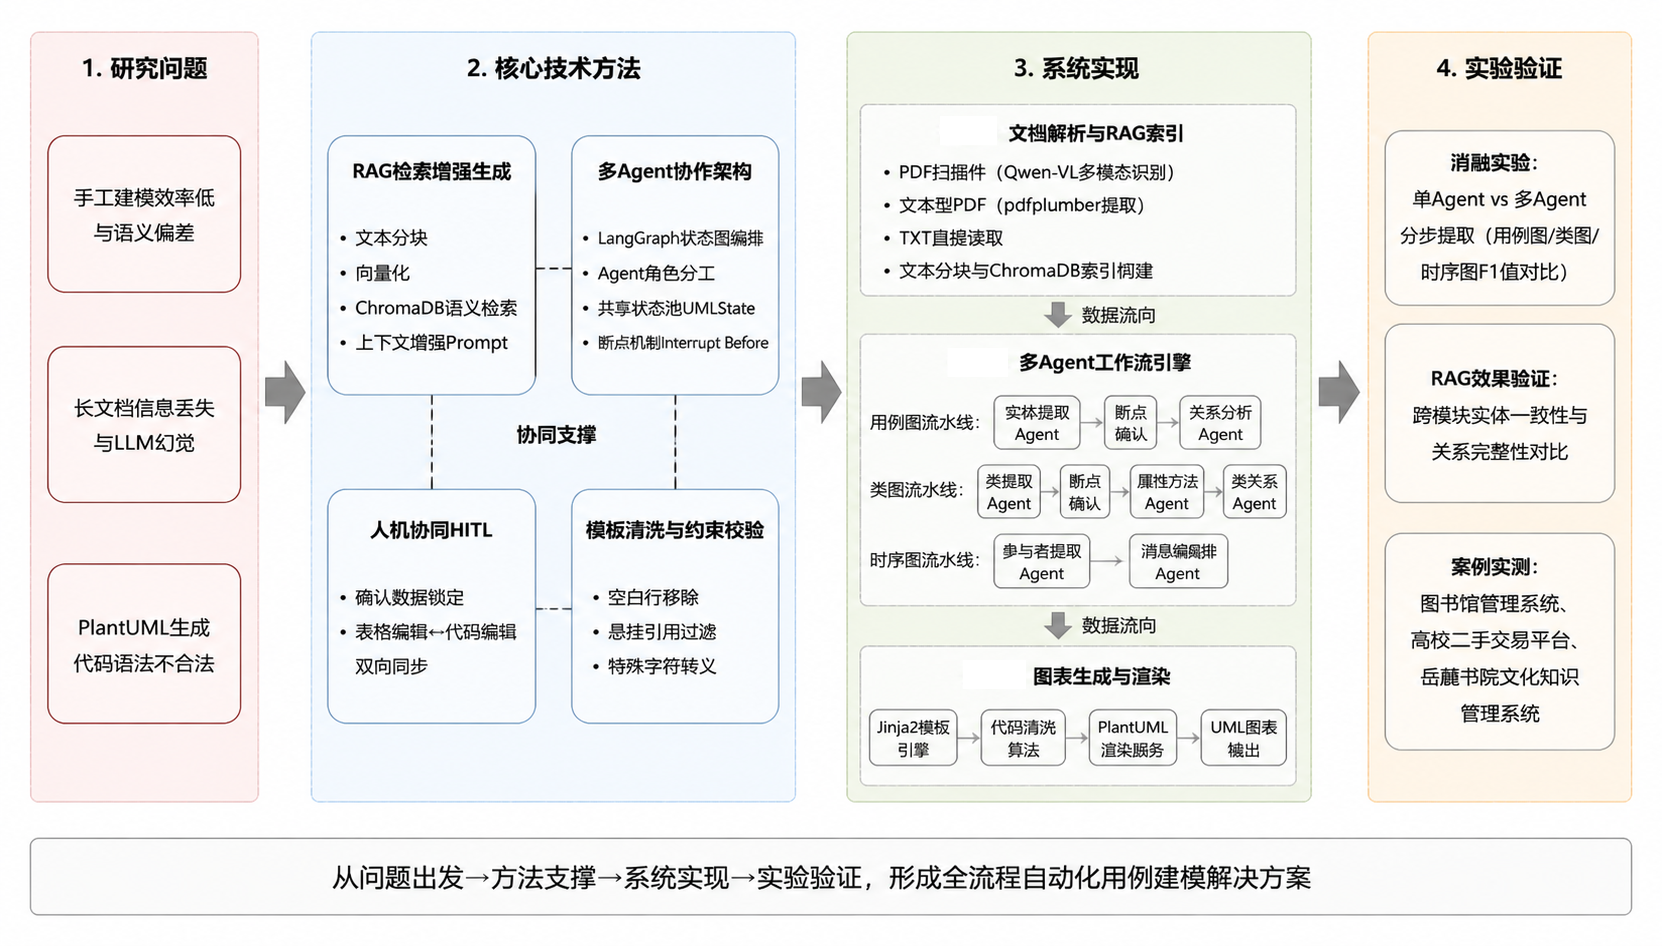
\includegraphics[width=150mm]{docs/imgs/技术路线图.png}
    \caption{论文技术路线图}
    \label{fig:tech_roadmap}
\end{figure}

\section{本章小结}

本章从软件工程实践中需求分析的重要性出发，分析了传统手工UML建模在效率、语义偏差和隐含关系识别方面存在的固有不足，指出大语言模型的语义理解能力为自动化建模带来了新的技术可能。在综述国内外研究现状的基础上，梳理了从传统NLP规则方法到LLM驱动建模再到多智能体协作系统的技术演进路径，明确了当前研究在长文档处理、幻觉抑制和多类型图表协同生成等方面仍面临的挑战。最后提出了本文的三项核心研究内容——构建基于LangGraph的多Agent协同建模管道、引入RAG技术缓解长文档信息丢失与幻觉问题、提出PlantUML模板清洗与逻辑约束算法，并说明了全文的章节组织安排。下一章将对系统所涉及的关键技术进行详细阐述，为后续章节的设计与实现提供理论基础。